\begin{frame}
    \frametitle{Estratégias de Otimização do Treinamento}

    \begin{block}{Votação}
        \begin{itemize}
            \item Resultados com menor variação de AUC;
            \item Execuções pouco mais longas;
        \end{itemize}
    \end{block}

    \begin{block}{Pares por instância}
        \begin{itemize}
            \item Resultados com maior variação de AUC;
            \item Restrição do tempo de execução;
        \end{itemize}
    \end{block}
\end{frame}

\begin{frame}
    \frametitle{Naïve Bayes}
    
    \begin{itemize}
        \item Resultados péssimos para as bases: Breast-Cancer, Hepatitis e Vehicle;
        \item Resultado ruim para a base: Glass;
        \item Resultado excelente para a base Yeast (Principalmente usando votação e amostragem);
        \item Comportamento bipolar não esclarecido.
    \end{itemize}
    
    \begin{figure}[H]
        \centering
        \subfloat[Breast cancer]{
            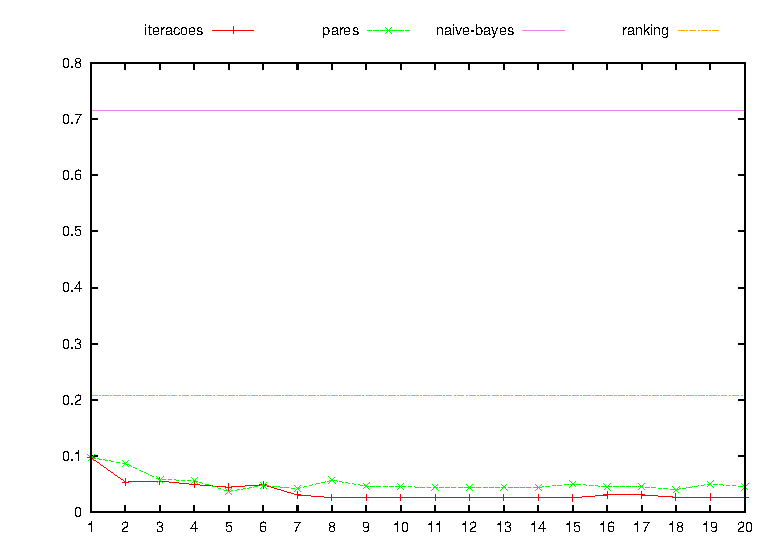
\includegraphics[width=0.3\textwidth]{img/breast-cancer_naive-bayes.eps}
        }
        \subfloat[Glass]{
            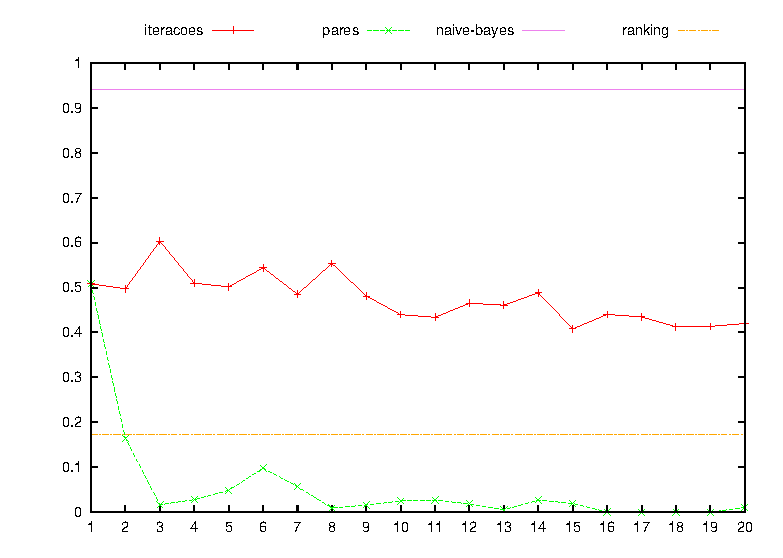
\includegraphics[width=0.3\textwidth]{img/glass_naive-bayes.eps}
        }
        \subfloat[Yeast]{
            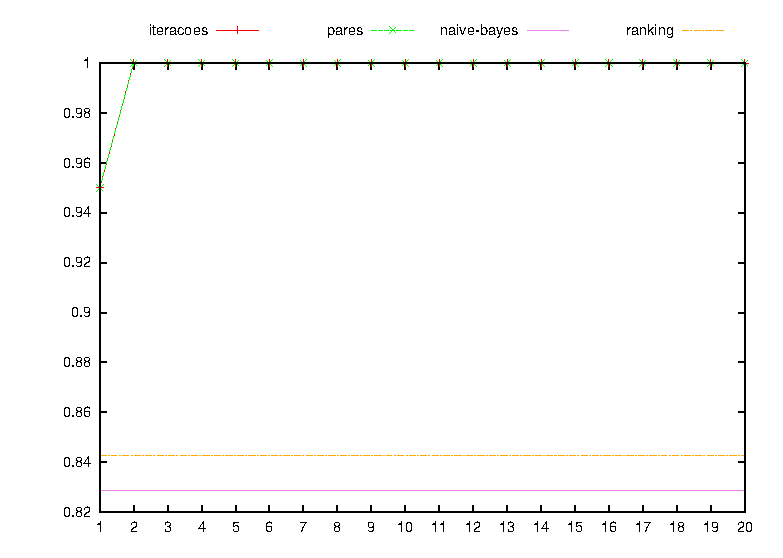
\includegraphics[width=0.3\textwidth]{img/yeast_naive-bayes.eps}
        }

        \caption{Gráficos de desempenho para Naïve Bayes}
    \end{figure}
\end{frame}

\begin{frame}
    \frametitle{Resultados da Técnica de Ranking Reduzido a Classificação}

    \begin{itemize}
        \item Em pouco mais da metade dos casos, a técnica teve melhores resultados sobre o classificador solo;
        \item Com a árvore de decisão C4.5 e a base Yeast, a técnica obteve uma melhora de aproximadamente 100\% sobre o classificador solo;
        \item A otimização de votação produziu resultados melhores que o classificador solo na maioria dos casos.
    \end{itemize}

    \begin{figure}[H]
        \centering
        \subfloat[C4.5 com a base Yeast]{
            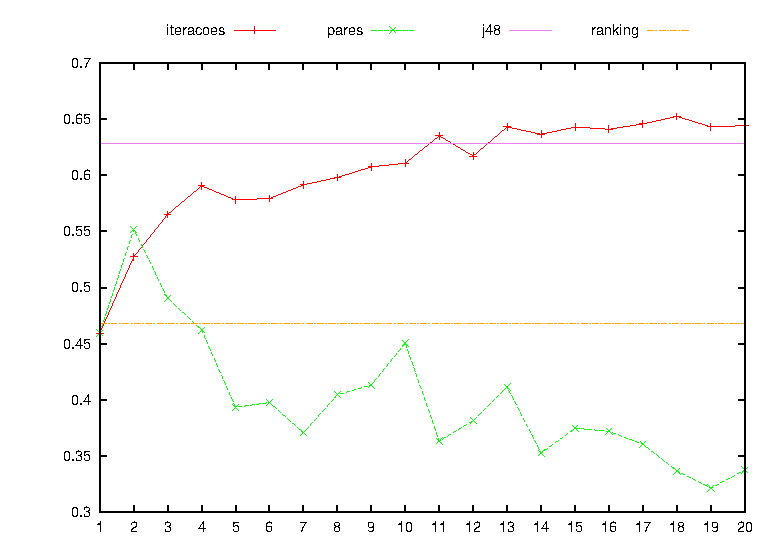
\includegraphics[width=0.45\textwidth]{img/breast-cancer_j48.eps}
        }
        \subfloat[SVM com a base Hepatitis]{
            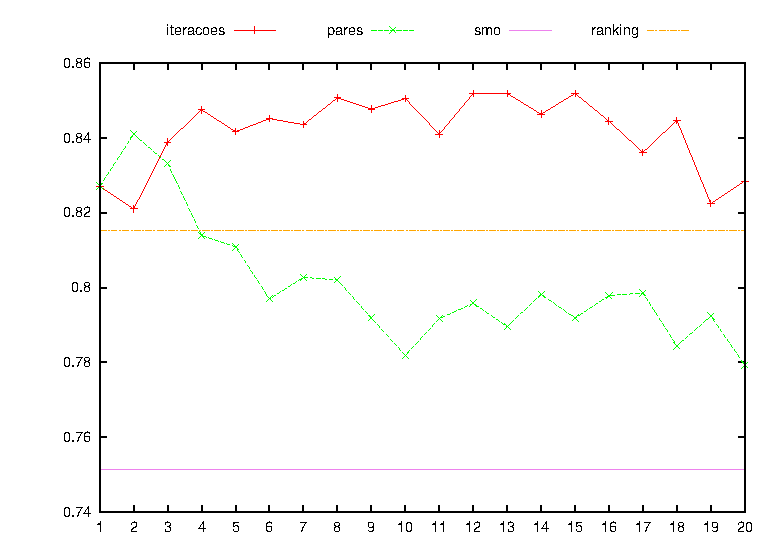
\includegraphics[width=0.45\textwidth]{img/hepatitis_smo.eps}
        }
        \caption{Gráficos de desempenho}
    \end{figure}
\end{frame}